\chapter{Results}\label{chp:results}

In this chapter, we present the results of different networks. Every section from \ref{sec:res} to \ref{sec:gogl} presents the results for each network. every section is divided in three subsection: one in which we discuss the results of different initialization one where we discuss the results of different optimizers and one in which the results for different classes are presented. 
\section{Resnet}\label{sec:res}
\subsection{Initialization}
For every class, we tested our network with either random initialization or with using pretrained weights. In Table \ref{tab:resinit}, we can see the best accuracy on validation set and the number of epochs for training for each class.  

\begin{table}
\caption{\label{tab:resinit} The results of training ResNet18 using random initialization or pretrained weights with Adamax as optimizer}
\centering
\begin{tabular}[b]{| l | l | l | l | l |}
\hline
    Initialization & Class & Validation accuracy (F1-score) & Epochs\ \\ \hline
    \multirow{}{}{Pretrained Weights} & Dunham &  62\%  & 50 \\ 
    & Porosity & 74\%  &  60 \\
    &DRT & 55\% &  50 \\
    &Components & 70\% &  50 \\ \hline
     \multirow{}{}{Random} & Dunham &  45\%  & 50 \\
    & Porosity & 64\% &  50 \\
    &DRT & 28\% & 50 \\
    &Components & 34\% &  50 \\ \hline
    
\end{tabular} 
\end{table}
On Figure\ref{fig:plotsres}, we plotted the accuracy, F1 score, and average training and validation loss for each class. 



\begin{figure}
\begin{subfigure}{.5\textwidth}
  \centering
  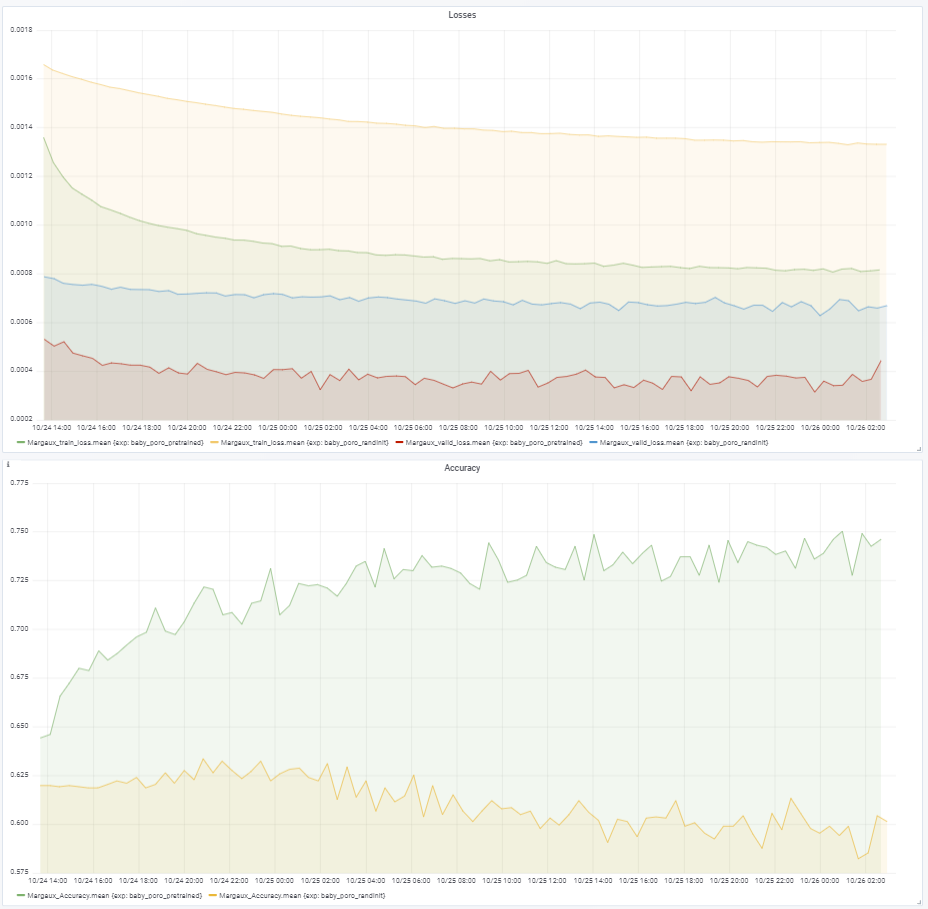
\includegraphics[width=.8\linewidth]{figures/04-Init_poro_acc.PNG}
  \caption{Resnet18 trained on the Porosity class.}
  \label{fig:resinit_poro}
\end{subfigure}%
\begin{subfigure}{.5\textwidth}
  \centering
  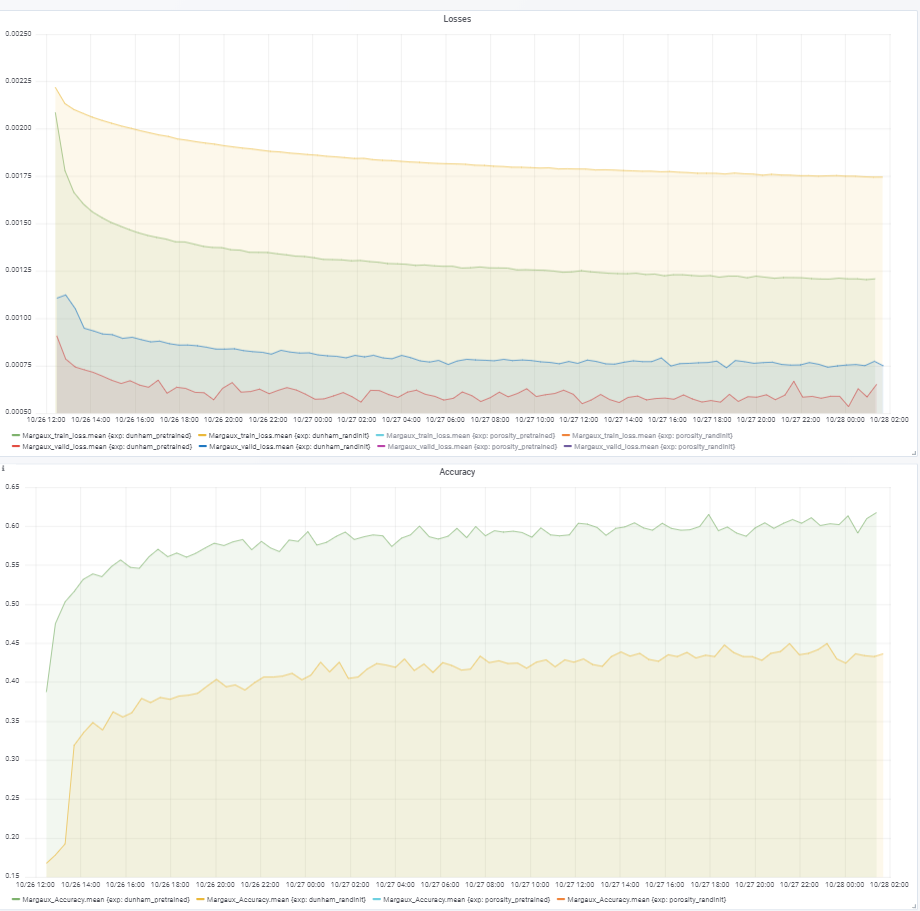
\includegraphics[width=.8\linewidth]{figures/04-Init_dunham_acc.PNG}
  \caption{Resnet18 trained on the Dunham class.}
  \label{fig:resinit_dunham}
\end{subfigure}
\begin{subfigure}{.5\textwidth}
  \centering
  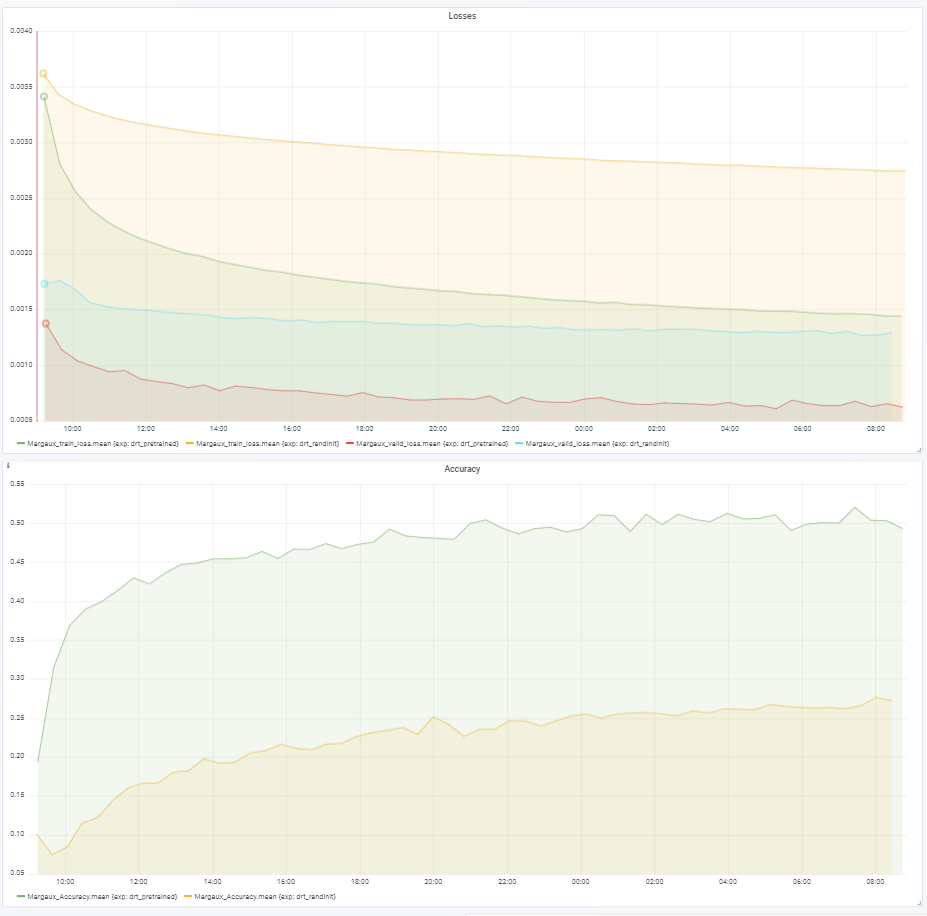
\includegraphics[width=.8\linewidth]{figures/04-Init_drt_acc.PNG}
  \caption{Resnet18 trained on the DRT class.}
  \label{fig:resinit_drt}
\end{subfigure}%
\begin{subfigure}{.5\textwidth}
  \centering
  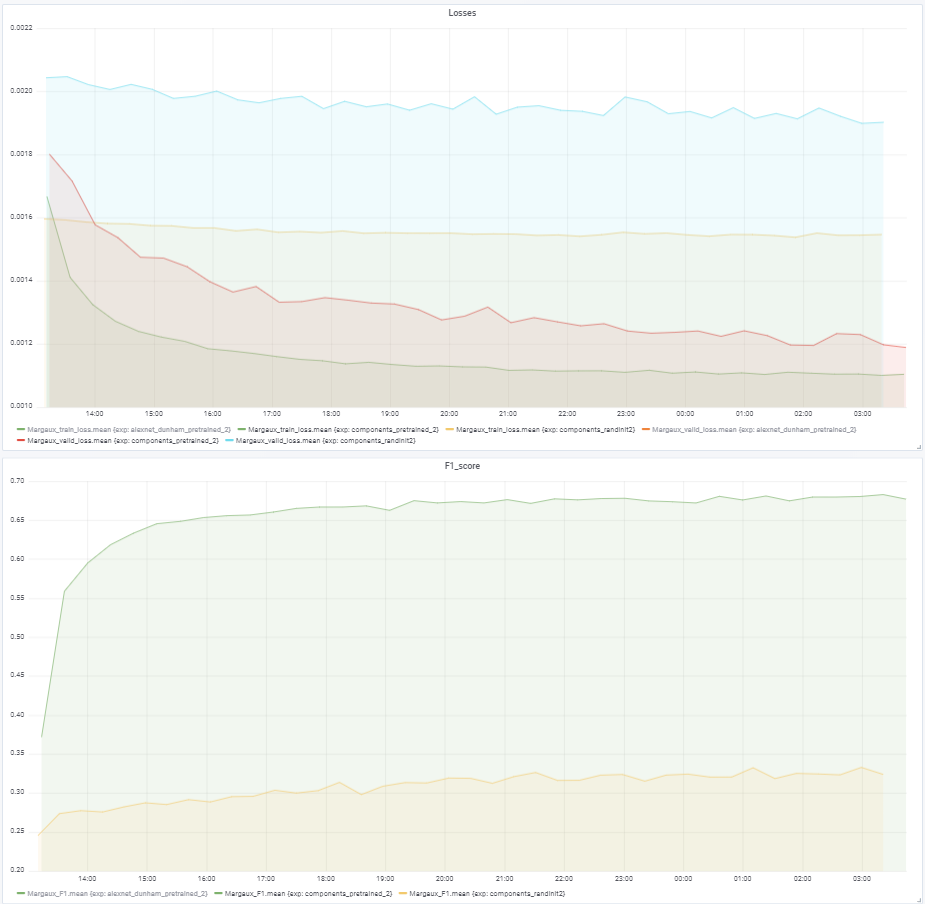
\includegraphics[width=.8\linewidth]{figures/04-Init_components_acc.PNG}
  \caption{Resnet18 trained on the Components class.}
  \label{fig:resinit_compo}
\end{subfigure}
\caption{The lines in green and red are for pretrained weights and yellow and blue for random initialization. The top plot is the validation accuracy for plots (a) (b) and (c) and the F1-score for plot (d), and the bottom plot is training  and validation loss.}
\label{fig:plotsres}
\end{figure}
\subsection{Classification}
On Table\ref{tab:resbest}, we summarize the best validation and test accuracy or F-1 score for every class. Then we present the confusion matrix for the best performing model and the test data set for the single label classification on Figure\ref{fig:rescm}. For the Components class, we show the statistics for every class. 

\begin{table}
\caption{\label{tab:resbest} The results of the best version of the Resnet 18 on the classification task. The validation and test accuracy are used as first metrics on the single label classification while F1-scores are used for multi-label classification.}
\centering
\begin{tabular}[b]{| l | l | l | l | l |}
\hline
    Initialization & Class & Validation accuracy (F1-score) & Test accuracy (F1-score) \ \\ \hline
    Pretrained Weights & Dunham &  62\%  & 38\% \\ \hline
    Pretrained Weights & Porosity & 74\%  &  58\% \\ \hline
    Pretrained Weights &DRT & 56\% &  25\% \\ \hline
    Pretrained Weights &Components & 69\% &  45\% \\ \hline
\end{tabular} 
\end{table}

\begin{figure}
\begin{subfigure}{.5\textwidth}
  \centering
  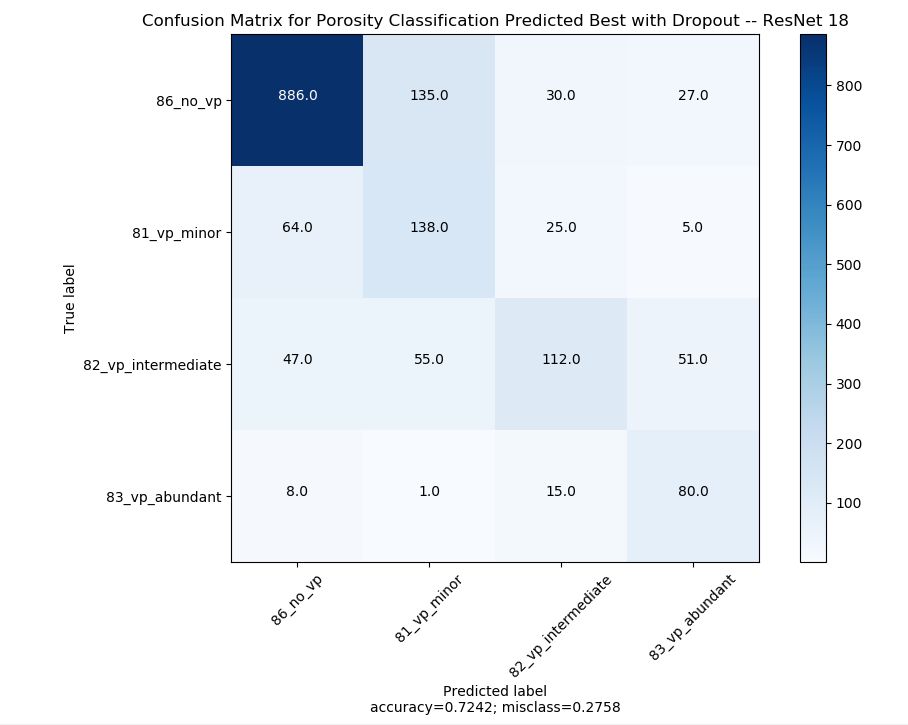
\includegraphics[width=.8\linewidth]{figures/04-baby_best.PNG}
  \caption{Best for Porosity}
  \label{fig:rescm_poro}
\end{subfigure}%
\begin{subfigure}{.5\textwidth}
  \centering
  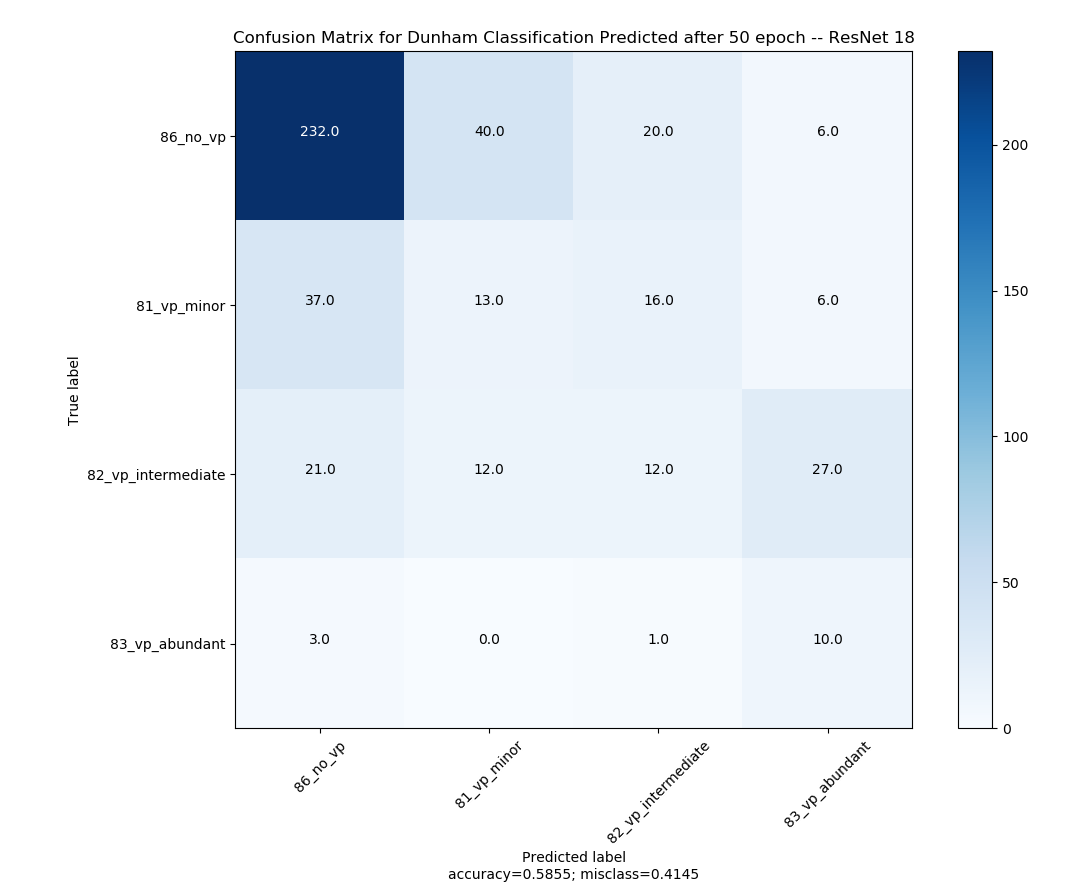
\includegraphics[width=.8\linewidth]{figures/04-baby_pred.PNG}
  \caption{Predicted for Porosity}
  \label{fig:rescmpred_poro}
\end{subfigure}
\begin{subfigure}{.5\textwidth}
  \centering
  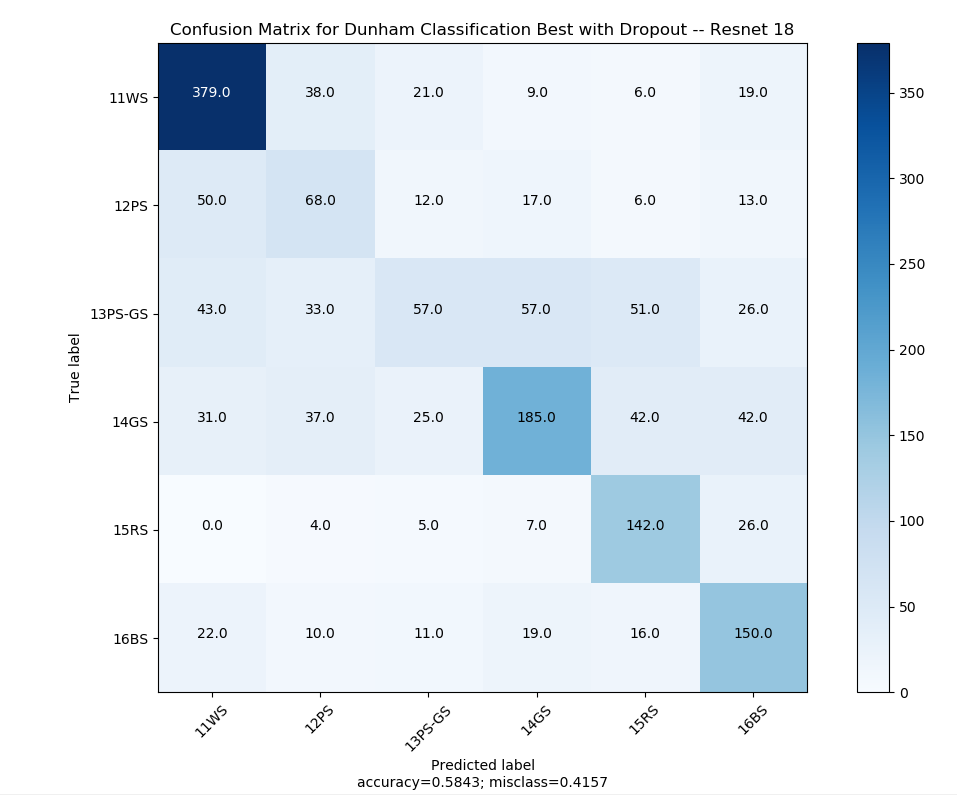
\includegraphics[width=.8\linewidth]{figures/04-dunham_best.PNG}
  \caption{Best for Dunham}
  \label{fig:rescm_dunham}
\end{subfigure}%
\begin{subfigure}{.5\textwidth}
  \centering
  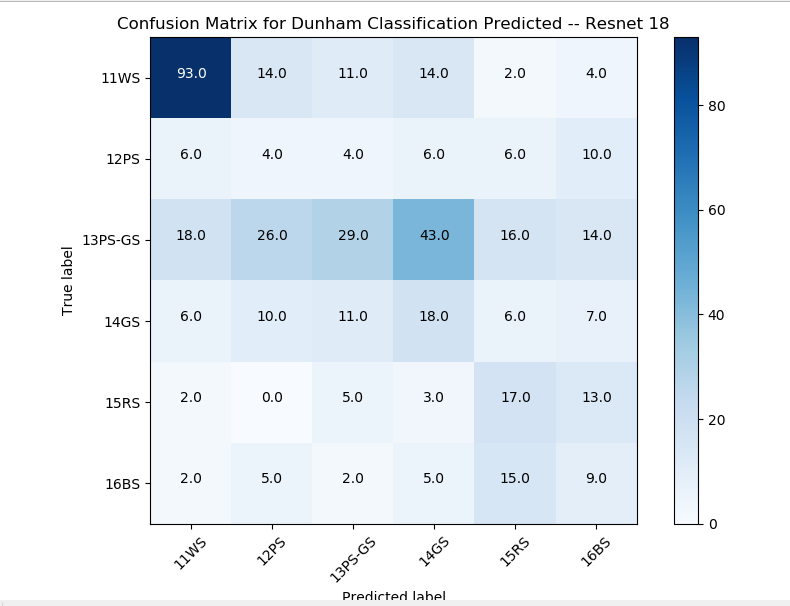
\includegraphics[width=.8\linewidth]{figures/04-dunham_pred.PNG}
  \caption{Predicted for Dunham}
  \label{fig:rescmpred_dunham}
\end{subfigure}
\begin{subfigure}{.5\textwidth}
  \centering
  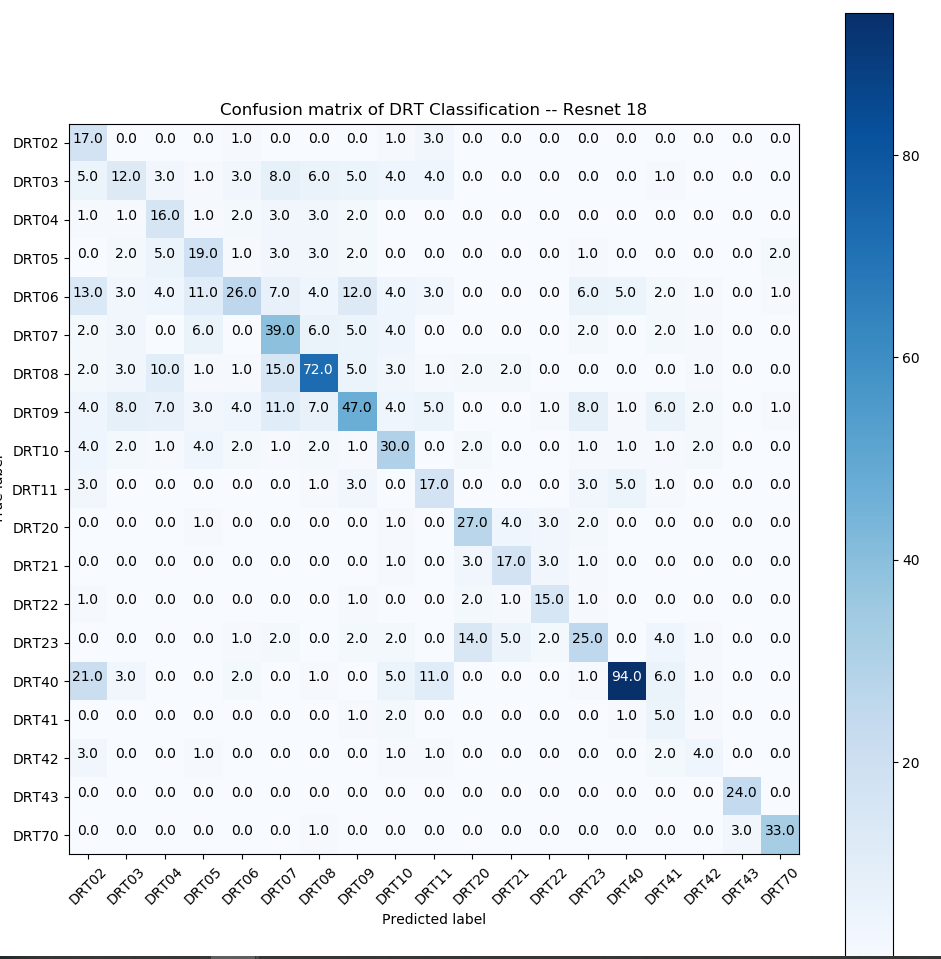
\includegraphics[width=.8\linewidth]{figures/04-DRT_best.PNG}
  \caption{Best for DRT}
  \label{fig:rescm_drt}
\end{subfigure}%
\begin{subfigure}{.5\textwidth}
  \centering
  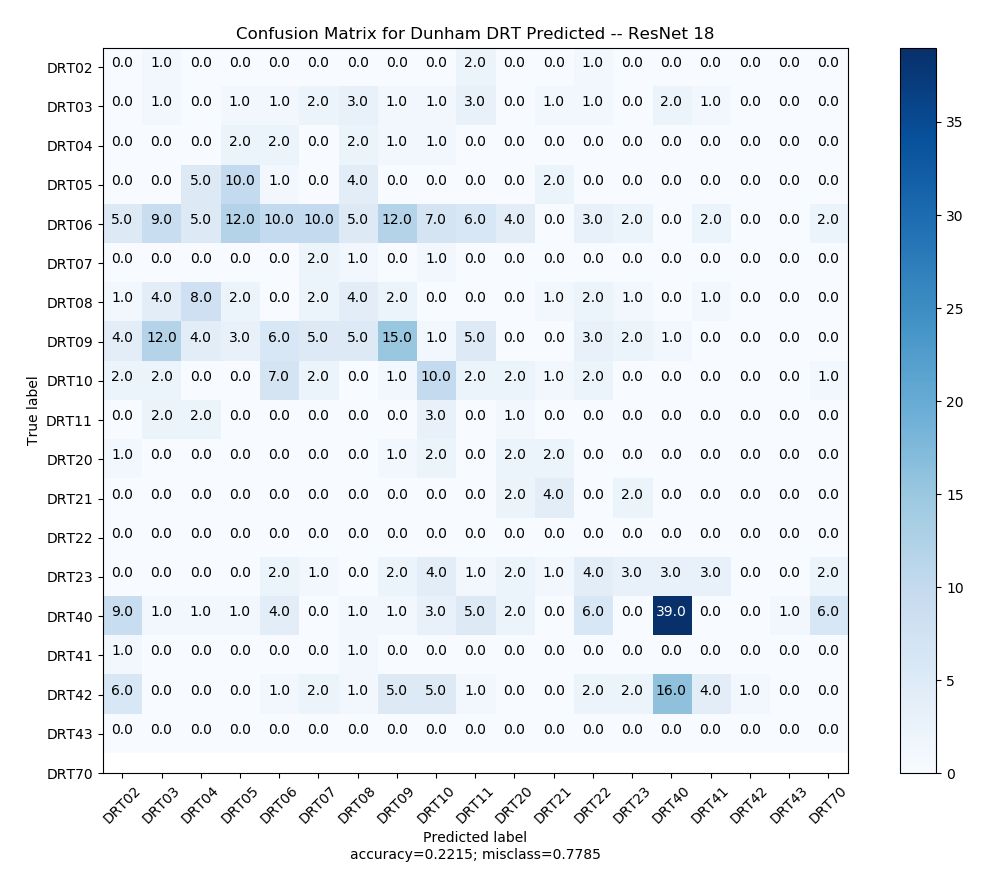
\includegraphics[width=.8\linewidth]{figures/04-drt_predicted.PNG}
  \caption{Predicted for DRT}
  \label{fig:rescmpred_drt}
\end{subfigure}
\caption{On the left is the confusion matrix of the best performing ResNet18 and on the right is the confusion matrix on the test set.}
\label{fig:rescms}
\end{figure}


%%%%%%%%%%%%%%%%%%%%%%%%%%%%%%%%%%%%%%%%%%%%%%%%%%%   ALEX   %%%%%%%%%%%%%%%%%%%%%%%%%%%%%%%%%%%%%%%%%%%%%%%%%%%%%

\section{AlexNet}\label{sec:aleX}
\subsection{Initialization}
For every class, we tested our network with either random initialization or with using pretrained weights. In Table \ref{tab:alexinit}, we can see the best accuracy on validation and test set, the number of epochs for training for each class.  
On Figure\ref{fig:plotsalex}, we plotted the accuracy, F1 score, and average training and validation loss for each class. 
\begin{table}
\caption{\label{tab:alexinit} The results of training AlexNet using random initialization or pretrained weights with Adamax as optimizer}
\centering
\begin{tabular}[b]{| l | l | l | l | l |}
\hline
    Initialization & Class & Validation accuracy  & Epochs\ \\ \hline
    \multirow{}{}{Pretrained Weights} & Dunham &  82\%  & 50 \\ %%cf Confusion Matrix 
    & Porosity & 89\% &  50 \\
    &DRT & 66\% &  50 \\
    &Components & 75\% &  50 \\ \hline
     \multirow{}{}{Random} & Dunham &  62\% & 50 \\
    & Porosity & 65\% &  50 \\
    &DRT & 61\% &  50 \\
    &Components & 75\% & 50 \\ \hline
\end{tabular} 
\end{table}

\begin{figure}
\begin{subfigure}{.5\textwidth}
  \centering
  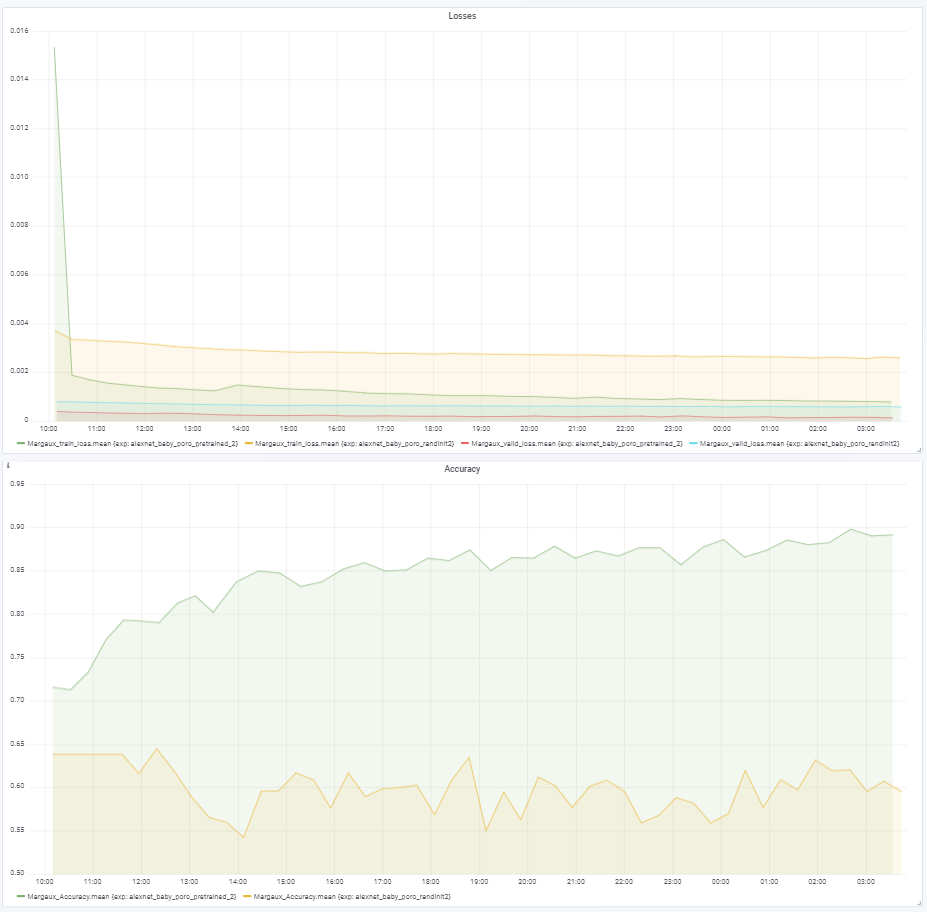
\includegraphics[width=.8\linewidth]{figures/04-Init_al_poro_acc.PNG}
  \caption{AlexNet trained on the Porosity class.}
  \label{fig:alexinit_poro}
\end{subfigure}%
\begin{subfigure}{.5\textwidth}
  \centering
  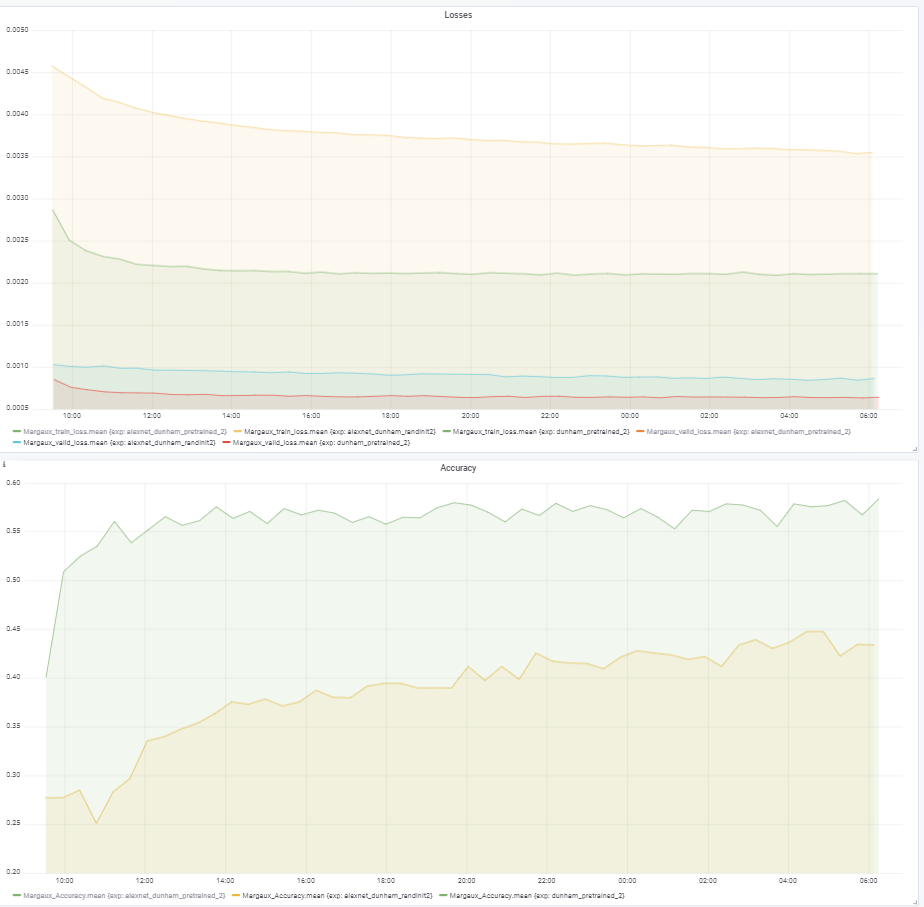
\includegraphics[width=.8\linewidth]{figures/04-Init_al_dunham_acc.PNG}
  \caption{AlexNet trained on the Dunham class.}
  \label{fig:alexinit_dunham}
\end{subfigure}
\begin{subfigure}{.5\textwidth}
  \centering
  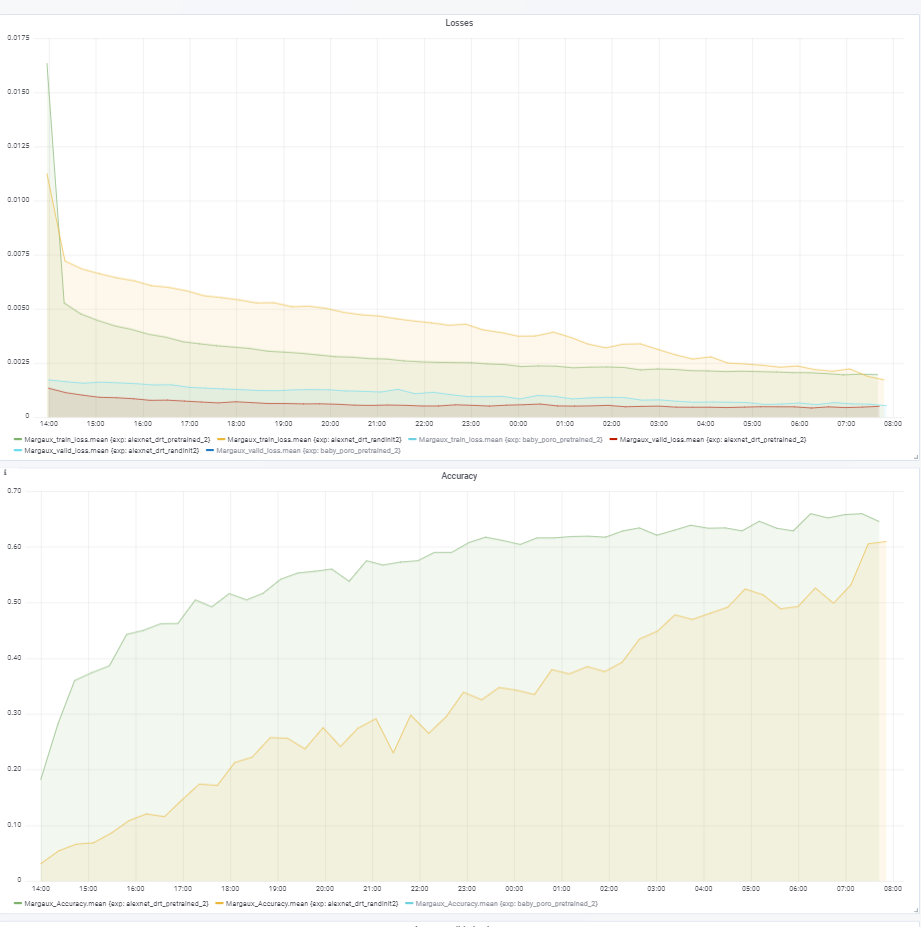
\includegraphics[width=.8\linewidth]{figures/04-Init_al_drt_acc.PNG}
  \caption{AlexNet trained on the DRT class.}
  \label{fig:alexinit_drt}
\end{subfigure}%
\begin{subfigure}{.5\textwidth}
  \centering
  \includegraphics[width=.8\linewidth]{figures/04-Init_al_components_acc.PNG}
  \caption{AlexNet trained on the Components class.}
  \label{fig:alexinit_compo}
\end{subfigure}
\caption{The lines in green and red are for pretrained weights and yellow and blue for random initialization. The top plot is the validation accuracy for plots (a) (b) and (c) and the F1-score for plot (d), and the bottom plot is training  and validation loss.}
\label{fig:plotsalex}
\end{figure}

\subsection{Classification}
On Table\ref{tab:ralexbest}, we summarize the best validation and test accuracy or F-1 score for every class. Then we present the confusion matrix for the best performing model and the test data set for the single label classification on Figure\ref{fig:alexcm}. For the Components class, we show the statistics for every class. 

\begin{table}
\caption{\label{tab:alexbest} The results of the best version of the AlexNet on the classification task. The validation and test accuracy are used as first metrics on the single label classification while F1-scores are used for multi-label classification.}
\centering
\begin{tabular}[b]{| l | l | l | l | l |}
\hline
    Initialization & Class & Validation accuracy (F1-score) & Test accuracy (F1-score) \ \\ \hline
    Pretrained Weights & Dunham &  82\%  & 39\% \\ \hline
    Pretrained Weights & Porosity & 89\%  &  69\% \\ \hline
    Pretrained Weights &DRT & 100\% &  100\% \\ \hline
    Pretrained Weights &Components & 100\% &  100\% \\ \hline
\end{tabular} 
\end{table}

\begin{figure}
\begin{subfigure}{.5\textwidth}
  \centering
  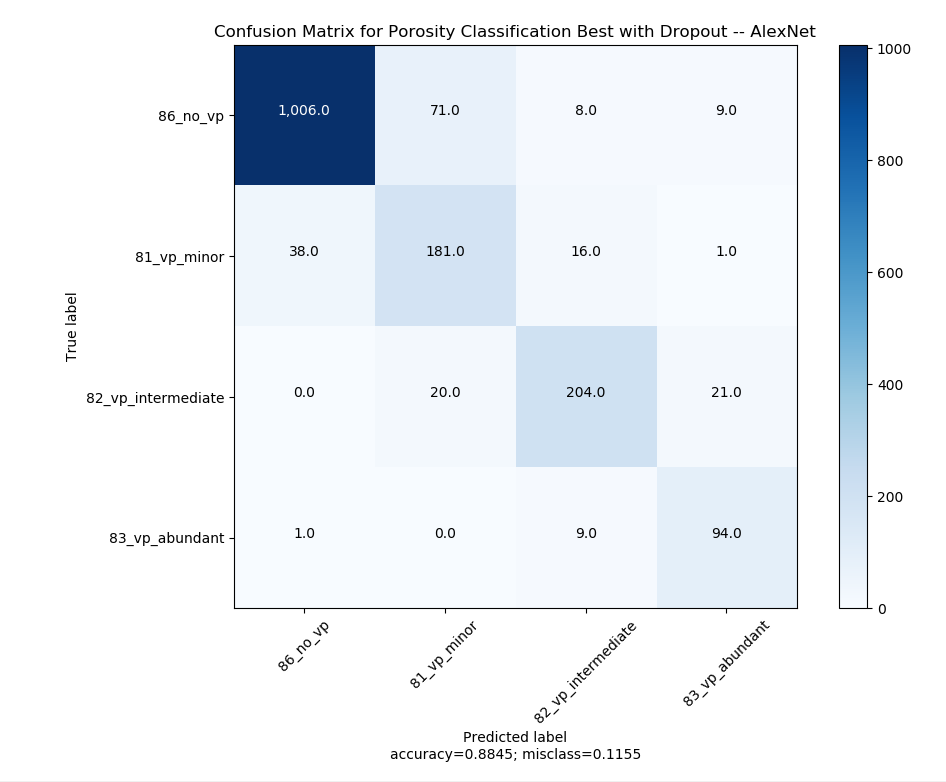
\includegraphics[width=.8\linewidth]{figures/04-al_baby_best.PNG}
  \caption{Best for Porosity}
  \label{fig:rescm_poro}
\end{subfigure}%
\begin{subfigure}{.5\textwidth}
  \centering
  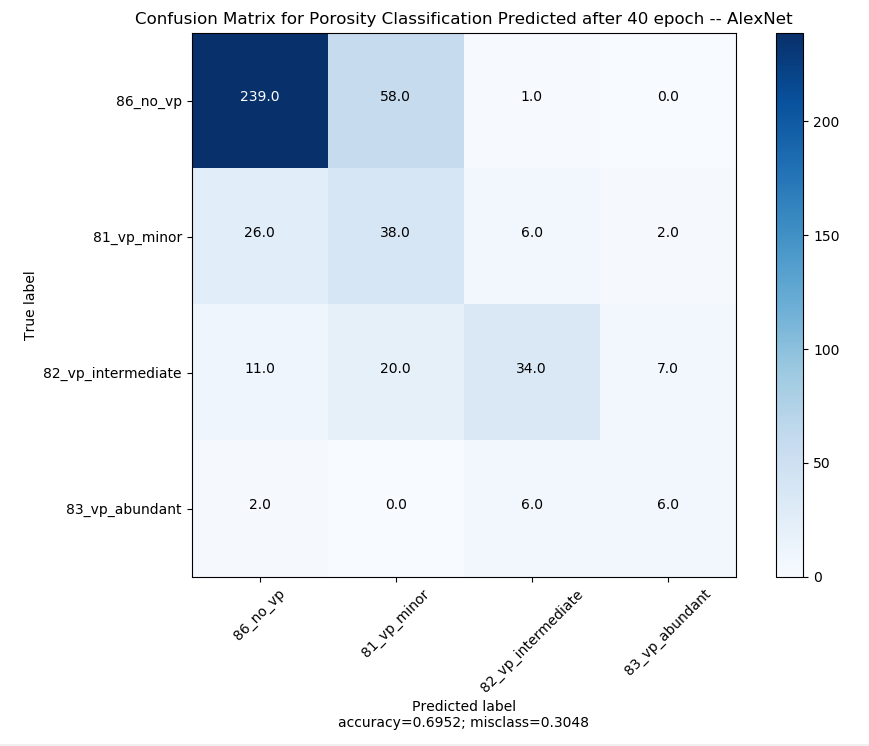
\includegraphics[width=.8\linewidth]{figures/04-al_baby_pred.PNG}
  \caption{Predicted for Porosity}
  \label{fig:rescmpred_poro}
\end{subfigure}
\begin{subfigure}{.5\textwidth}
  \centering
  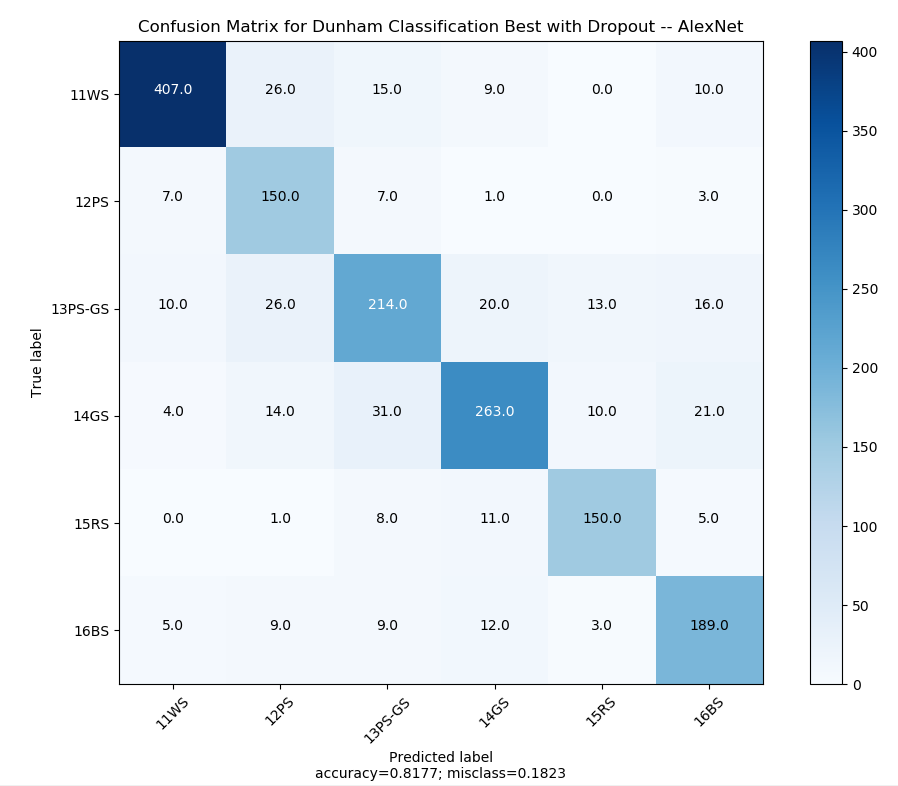
\includegraphics[width=.8\linewidth]{figures/04-al_dunham_best.PNG}
  \caption{Best for Dunham}
  \label{fig:rescm_dunham}
\end{subfigure}%
\begin{subfigure}{.5\textwidth}
  \centering
  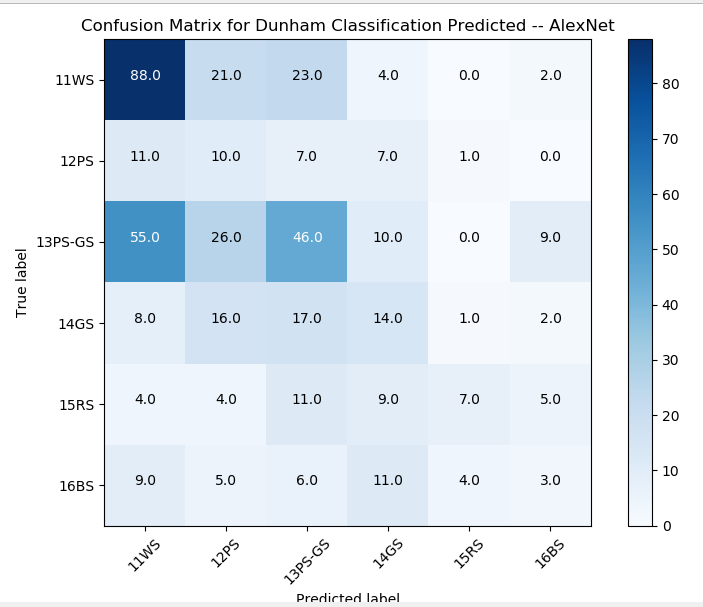
\includegraphics[width=.8\linewidth]{figures/04-al_dunham_predicted.PNG}
  \caption{Predicted for Dunham}
  \label{fig:rescmpred_dunham}
\end{subfigure}
\begin{subfigure}{.5\textwidth}
  \centering
  \includegraphics[width=.8\linewidth]{figures/04-al_DRT_best.PNG}
  \caption{Best for DRT}
  \label{fig:rescm_drt}
\end{subfigure}%
\begin{subfigure}{.5\textwidth}
  \centering
  \includegraphics[width=.8\linewidth]{figures/04-al_drt_predicted.PNG}
  \caption{Predicted for DRT}
  \label{fig:rescmpred_drt}
\end{subfigure}
\caption{On the left is the confusion matrix of the best performing AlexNet and on the right is the confusion matrix on the test set.}
\label{fig:rescms}
\end{figure}


%%%%%%%%%%%%%%%%%%%%%%%%%%%%%%%%%%%%%%%%%%%%%%%%%%%   ALEX   %%%%%%%%%%%%%%%%%%%%%%%%%%%%%%%%%%%%%%%%%%%%%%%%%%%%%


\section{GoogleNet}\label{sec:gogl}
\subsection{Initialization}

\subsection{Classification}

\section{Optimizer}